\chapter{Problema}

Nuestro problema consiste en un robot, situado en un entorno parcialmente desconocido. Tenemos un objetivo, pero no 
sabemos lo suficiente sobre el entorno como para decidir si podemos satisfacerlo o no.
Debemos obtener el conocimiento necesario sobre el entorno para poder decidir sobre el objetivo. Para lograrlo, vamos
a utilizar los sensores del robot, los cuales nos aportan información, y una estrategia que utilice
el conocimiento que adquirido para obtener conocimiento nuevo.

\section{Definición}

La solución al problema de la síntesis de controladores en entornos desconocidos es un LTS x tal que M $\parallel$ x $\models$ G, 
en donde M es el MTS que modela el entorno y G son los objetivos de tipo GR(1). Mediante la síntesis de controladores sobre MTS,
podemos intentar generar automáticamente el x. La síntesis tiene tres escenarios posibles:

\begin{itemize}

\item
Si se puede sintetizar x para cualquier implementación de M, obtenemos el controlador que necesitamos, el cual es la
solución a nuestro problema.

\item
Si no se puede sintetizar x para ninguna implementación de M, sabemos que nuestro problema no tiene solución.

\item
Si se puede sintetizar x para algunas implementaciones de M, pero no se puede sintetizar para otras implementaciones de M,
no sabemos si es posible sintetizar un controlador para la implementación de M que representa al mundo real, la cual no conocemos.

\end{itemize}

\vspace{\baselineskip}
En los dos primeros escenarios tenemos una respuesta a nuestro problema. De estar en el tercer escenario, queremos poder sintetizar
el controlador en caso de ser posible, o tener garantías de que es imposible sintetizar dicho controlador. Para lograr nuestro objetivo
debemos agregar información a M, para poder reducir su cantidad de posibles implementaciones, y que de esta forma su síntesis caiga
en uno de los dos primeros escenarios.

\vspace{\baselineskip}
La exploración nos permite adquirir conocimiento, ya que al observar mediante los sensores del robot lugares del entorno en los cuales
no habíamos estado, podemos despejar la incertidumbre en nuestro modelo del entorno, representado por M. Vamos a realizar la exploración
mediante un algoritmo, el cual se basa en ciclos de adquisición de conocimiento. Si nuestra información sobre el entorno es insuficiente,
movemos al robot para que pueda aprender algo nuevo. Repetimos el ciclo hasta poder dar una respuesta.

\section{Algoritmo}

\begin{figure}[H]
  \centering
    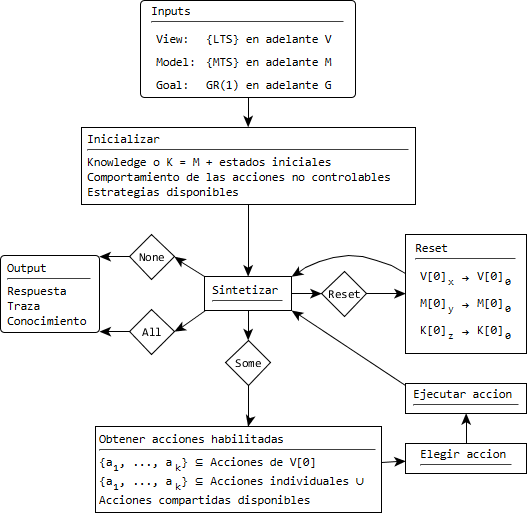
\includegraphics{Imagenes/Algoritmo/Algoritmo.png}
  \caption{Algoritmo de exploración}
  \label{fig:Algoritmo}
\end{figure}

\section{Inputs}

Para resolver el problema necesitamos poder observar al ambiente a medida que nos movemos, saber con que información inicial 
contamos y tener un objetivo que cumplir.

\subsection{View}
\textbf{View} es una lista de LTSs. Representa el mundo sobre el cual se mueve el robot.
El primer LTS de la lista representa el mapa del ambiente, el cual regula como se mueve el robot por el mundo. Indica que acciones
puede realizar en cada posición, y a que lugar lo llevan dichas acciones.
Los otros LTSs representan el comportamiento de los agentes externos que interactúan con el ambiente. Pueden bloquear y habilitar
acciones en una determinada posición. El robot no tiene influencia sobre ellos.
El robot solo puede observar el estado actual del \textbf{View} mediante sus sensores. Sobre el mapa, solo puede saber en que posición está
y que acciones puede ejecutar en dicha posición. Sobre los agentes externos, solo puede observar su estado actual.

\subsection{Model}
\textbf{Model} es una lista de MTSs. Representa nuestro conocimiento inicial sobre el mundo. Por cada LTS en \textbf{View} hay un correspondiente MTS
en \textbf{Model}.
La única restricción para los MTSs de \textbf{Model}, es que puedan refinarse en sus correspondientes LTSs de \textbf{View}. Por lo tanto, como mínimo,
cada MTS debe contar con un estado, y por cada acción en su correspondiente LTS, debe haber una acción posible en el MTS.

\subsection{Goal}
\textbf{Goal} es el objetivo del robot. Exploramos para poder decidir si es posible garantizar el cumplimiento de \textbf{Goal}. Esta expresado con una 
fórmula GR\big(1\big).

\section{Inicialización}

\textbf{Knowledge} es una lista de MTSs que representa el conocimiento que vamos adquiriendo en cada iteración del algoritmo. En cada iteración, los MTSs
de \textbf{Knowledge} son un refinamiento de los MTSs de la iteración anterior. Cada MTS de \textbf{Knowledge} se compone de dos grupos de estados: Los
que están en \textit{La nube} y los que representan el conocimiento.

\vspace{\baselineskip}
\textit{La nube} representa la incertidumbre. Es una copia del MTS de \textbf{Model}. Sus estados y acciones se mantienen inmutables en todas las 
iteraciones de \textbf{Knowledge}.
El resto de los estados representan el conocimiento adquirido hasta el momento. Su cantidad de estados ira creciendo a medida que el robot adquiera información.
En cada estado, las acciones que nunca fueron ejecutadas irán a un estado de \textit{La nube}, mientras que las que ya fueron ejecutadas, irán a un estado del
conocimiento.

\vspace{\baselineskip}
En la implementación del algoritmo en la herramienta MTSA, hay dos cuestiones importantes de inicialización.
Por un lado, el comportamiento de las acciones no controlables de los agentes externos. Actualmente existen dos patrones de comportamiento.
Por defecto, los agentes externos elegirán una acción al azar. El otro patrón de comportamiento consiste en que se comporten de forma cíclica ejecutando
las acciones que nosotros pasamos como input. En el futuro podrá extenderse la herramienta con más patrones de comportamiento.
La otra cuestión es la estrategia utilizada por el robot. En esta tesis presentamos una única estrategia que resuelve el problema, pero en el futuro puede
extenderse la herramienta con estrategias diferentes.

\section{Síntesis}

\begin{figure}[H]
  \centering
    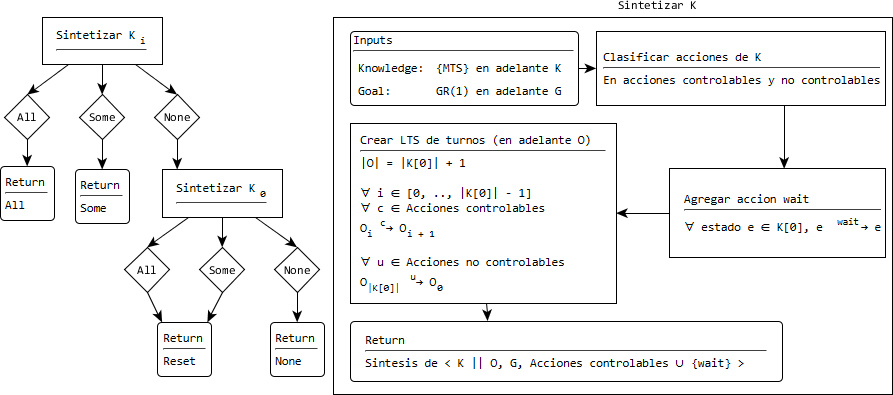
\includegraphics[width=1.0\textwidth]{Imagenes/Algoritmo/Algoritmo_sintetizar.png}
  \caption{Algoritmo de síntesis}
  \label{fig:Algoritmo_sintetizar}
\end{figure}

Al principio de cada iteración, lo primero que hacemos es intentar dar una respuesta a la pregunta sobre si podemos garantizar el cumplimiento del objetivo.
En otras palabras, queremos ver si podemos sintetizar un controlador que garantice el cumplimiento de \textbf{Goal}.

\vspace{\baselineskip}
La síntesis la haremos sobre un MTS basado en \textbf{Knowledge}, pero con algunas modificaciones necesarias para modelar correctamente el problema.
Primero cambiamos el estado inicial del primer MTS de \textbf{Knowledge}, el que representa el mapa, para que su estado inicial sea el estado en el que está
situado actualmente el robot. Esto es para que el controlador garantice el objetivo desde nuestra posición actual.

\vspace{\baselineskip}
Luego, al primer MTS de \textbf{Knowledge} (el mapa), le agregaremos en cada estado la acción controlable wait, que irá al mismo estado.
Esto es para representar la posibilidad de que el robot espere en su posición actual un cambio en los agentes externos.

\vspace{\baselineskip}
Por último creamos un LTS de turnos, que permita al robot moverse a cualquier estado antes de que los agentes externos realicen cambios. Esto es para evitar que los
agentes externos esperen que el robot este lejos para realizar una acción que beneficie al robot. El LTS de turnos permitirá que el robot se mueva una cantidad
de veces igual a la cantidad de estados del primer MTS del \textbf{Knowledge} (el mapa) antes de que los agentes externos se muevan.

\vspace{\baselineskip}
De esta forma, con la posibilidad de moverse y esperar en cualquier estado conocido, puede estar en el estado necesario para beneficiarse de las acciones de
los agentes externos. Sintetizaremos el controlador para \textbf{Goal} sobre la composición en paralelo de los MTSs de \textbf{Knowledge}, incluyendo el MTS al
cual le agregamos las acciones wait, con el LTS de turnos.

\vspace{\baselineskip}
Si el resultado de la síntesis es que puede generarse un controlador para cualquier LTS que sea un refinamiento del MTS que armamos, significa que el robot
puede cumplir el objetivo sin importar como sean las zonas inexploradas del entorno. El algoritmo termina, dando como resultado la garantía del cumplimiento
de \textbf{Goal}.

\vspace{\baselineskip}
En caso de que no pueda generarse un controlador mara ningún LTS que sea un refinamiento del MTS que armamos, hay que volver a realizar la síntesis, pero sin
realizar el cambio del estado inicial. Si nuevamente no puede generarse un controlador, significa que es imposible cumplir \textbf{Goal}, sin importar como sean
las zonas inexploradas del entorno, y el algoritmo termina confirmando la imposibilidad de cumplimiento de \textbf{Goal}. En caso contrario, significa que
llegamos a un punto sin retorno, pero todavía hay zonas inexploradas que pueden ser alcanzadas desde el inicio, en las cuales podríamos o no cumplir el objetivo.

\vspace{\baselineskip}
En caso de que nuestro robot tenga la capacidad de volver al inicio, o utilizar otro robot desde la zona inicial, podemos seguir explorando cambiando los
estados iniciales de los primeros componentes de \textbf{View}, \textbf{Model} y \textbf{Knowledge} (los que representan al mapa) al estado inicial del comienzo
de la exploración. Al hacer esto contamos con la información recolectada hasta el momento, la cual puede utilizar la estrategia para no volver a caer en el
punto sin retorno.

\vspace{\baselineskip}
Por ultimo, si la síntesis puede generar un controlador para algunas de las implementaciones del MTS que armamos, pero para otras no, significa que no tenemos
suficiente información sobre el entorno como para decidir sobre el objetivo, y necesitamos seguir explorando para refinar el \textbf{Knowledge}.

\section{Estrategia Síntesis - Nueva acción}

\begin{figure}[H]
  \centering
    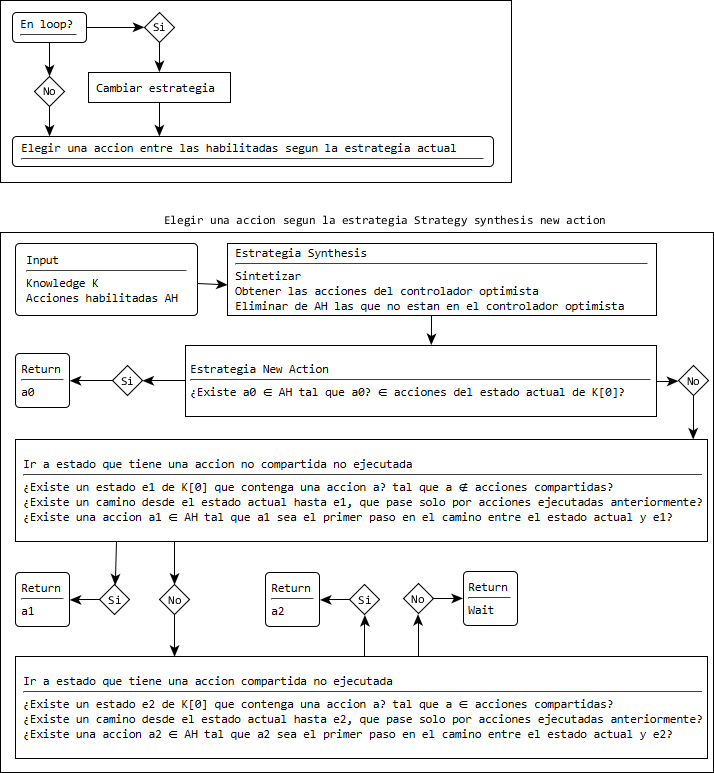
\includegraphics[width=1.0\textwidth]{Imagenes/Algoritmo/Algoritmo_elegir.png}
  \caption{Algoritmo de la estrategia Síntesis - Nueva acción}
  \label{fig:Algoritmo_elegir}
\end{figure}

En caso de que sea necesario seguir explorando, necesitamos que la estrategia decida la próxima acción a ejecutar. El algoritmo esta preparado para que,
al utilizar múltiples estrategias, detecte si alguna entra en un ciclo infinito y la reemplace por otra. En esta tesis vamos a presentar únicamente
la estrategia Síntesis - Nueva acción, la cual no entra en ciclos. Dicha estrategia es la composición de la estrategia Síntesis, que busca evitar caer
en zonas inseguras utilizando la información proporcionada por \textbf{Model}, y la estrategia Nueva acción, que busca siempre adquirir conocimiento nuevo
utilizando información proporcionada por \textbf{Knowledge}.

\vspace{\baselineskip}
Estamos por elegir una acción. Hacemos esto porque el intento de síntesis para generar un controlador que garantice \textbf{Goal} nos dio como resultado que
existe un controlador para algunos refinamientos pero no para otros. En particular existe un controlador para el refinamiento más optimista, llamado
controlador optimista. La estrategia Síntesis aprovecha este hecho, ya que por construcción, el controlador optimista evitara las zonas inseguras. Lo que
hace la estrategia es elegir de entre las acciones posibles, una acción que esté en el estado inicial del controlador optimista. En cambio, la estrategia
Síntesis - Nueva acción lo utiliza para filtrar de entre las acciones posibles, cuales son las acciones seguras, y así elegir mediante la estrategia Nueva acción
una acción entre las seguras.

\vspace{\baselineskip}
La estrategia Nueva acción tiene como objetivo ejecutar acciones nuevas, o en otras palabras, que no hayan sido ejecutadas anteriormente en su estado asociado.
Si siempre ejecutamos acciones nuevas, siempre adquiriremos conocimiento nuevo, y como el entorno a explorar es finito, terminaremos por reconocerlo completamente
de seguir esta estrategia.

\vspace{\baselineskip}
La estrategia se divide en varias etapas. Lo primero que debemos hacer es saber si, entre las acciones disponibles, existe alguna que no haya sido ejecutada
anteriormente desde el estado actual. Si existe, la eligiéremos, porque es una acción nueva.

\vspace{\baselineskip}
Si el estado actual es un estado completamente explorado, o en otras palabras, ya ejecutamos anteriormente todas las acciones disponibles desde este estado, debemos
llegar a un estado no completamente explorado. Para hacerlo, buscamos si hay algún estado que cumpla las condiciones deseadas al que podamos volver. Esto
significa que exista un estado con alguna acción controlable como posible, y que podamos llegar a el por un camino de acciones requeridas en el primer componente
de \textbf{Knowledge} (el mapa).

\vspace{\baselineskip}
Para construir el camino, sintetizaremos un controlador con el objetivo de llegar a ese estado desde nuestro estado actual. Para lograrlo construiremos un MTS
a partir del primer componente de \textbf{Knowledge}. Debemos agregar una acción ganadora al estado al que queremos llegar. El objetivo sera ejecutar dicha acción,
por lo cual para lograrlo tenemos que llegar al estado deseado desde nuestro estado actual. El segundo paso es eliminar las acciones posibles, para que el camino
solo esté compuesto por acciones requeridas, o en otras palabras, ya ejecutadas anteriormente. En caso de existir el controlador buscado, necesitamos que el camino
comience por alguna de las acciones disponibles desde nuestro estado actual. Si ese es el caso, la elegimos, porque nos acerca a una acción nueva.

\vspace{\baselineskip}
Si no existen estados con acciones controlables no ejecutadas anteriormente, lo que tenemos que hacer es llegar a un estado con una acción compartida no ejecutada
anteriormente, y esperar a que los agentes externos nos permitan ejecutarla. Seguimos el mismo procedimiento de síntesis utilizado anteriormente. Si existe el camino,
elegimos la acción que nos permita acercarnos, en caso contrario eligiéremos esperar, ya que es necesaria la interacción de algún agente externo para poder continuar
explorando.

\section{Ejecución}

\begin{figure}[H]
  \centering
    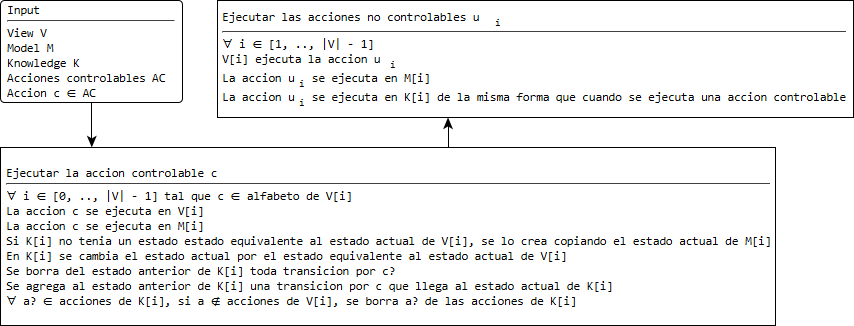
\includegraphics[width=1.0\textwidth]{Imagenes/Algoritmo/Algoritmo_ejecutar.png}
  \caption{Algoritmo de ejecución}
  \label{fig:Algoritmo_ejecutar}
\end{figure}

Al ejecutar la acción elegida, el robot puede, o no, cambiar de ubicación en el entorno. Esto implica un cambio en el estado actual de la primer componente tanto 
de \textbf{View}, como de \textbf{Model} y \textbf{Knowledge}. La primer componente de \textbf{Knowledge} también puede cambiar su estructura, refinando el MTS,
como consecuencia de la nueva información aportada por los sensores del robot en su nueva ubicación.

\vspace{\baselineskip}
Si es la primera vez que el robot se encuentra en la ubicación actual, se va a agregar un nuevo estado en la primer componente de \textbf{Knowledge}, en el que todas
sus acciones se dirigen hacia \textit{La nube}. En caso de haber ejecutado una acción que se dirigía hacia \textit{La nube}, ahora podemos observar a que ubicación
en el entorno nos lleva, por lo cual vamos a poder transformar en nuestro modelo dicha acción en una acción requerida que va hacia el estado correspondiente
a la ubicación actual.

\vspace{\baselineskip}
Luego de ejecutar la acción elegida, hay que ejecutar las acciones ejecutadas por los agentes externos. Los cambios en los agentes externos afectan el estado actual
de las restantes componentes de \textbf{View}, \textbf{Model} y \textbf{Knowledge}, y la estructura de las restantes componentes de \textbf{Knowledge}. El proceso se
realiza en la forma descripta por la figura 3.4.

\section{Ciclo de exploración}

\begin{figure}[H]
  \centering
    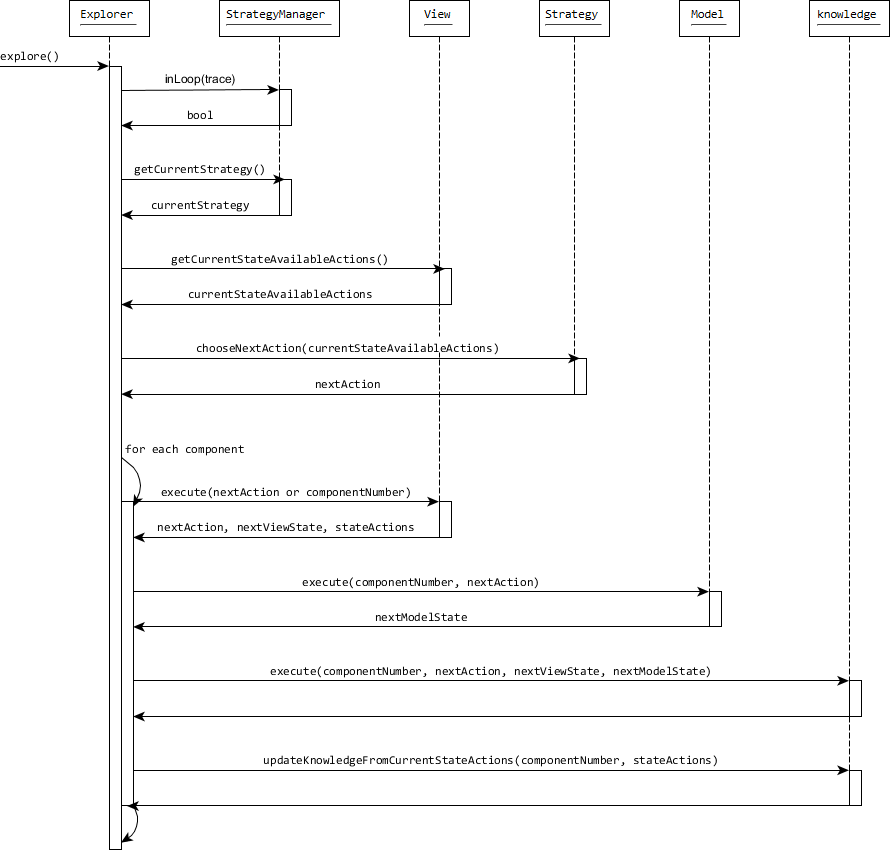
\includegraphics[width=1.0\textwidth]{Imagenes/Algoritmo/Secuencia_explorar.png}
  \caption{Diagrama de secuencia}
  \label{fig:Secuencia_explorar}
\end{figure}

La figura 3.5 nos muestra como interactúan los diferentes objetos durante un ciclo de exploración.

\vspace{\baselineskip}
Lo primero que hacemos es comprobar que la estrategia actual no haya entrado en un ciclo, ya que de no visitar estados nuevos no puede aportar información nueva.

\vspace{\baselineskip}
En caso de que la estrategia actual este en un ciclo la reemplazamos por otra. Una vez que tenemos la estrategia adecuada, observamos mediante los sensores que
acciones tenemos disponibles en la ubicación actual, con el estado actual de los agentes externos. Le pedimos a la estrategia que elija una acción entre las
acciones disponibles.

\vspace{\baselineskip}
Cuando tenemos definida la siguiente acción, necesitamos ejecutarla. Primero la ejecutamos en \textbf{View}. Al hacerlo podemos sensar en que ubicación nos
encontramos y que acciones tenemos disponibles.

\vspace{\baselineskip}
Luego la ejecutamos en \textbf{Model}, para que su estado actual se corresponda al estado que modela al estado actual de \textbf{View}.

\vspace{\baselineskip}
A continuación ejecutamos la acción en \textbf{Knowledge}, y en caso de que la acción vaya a un nuevo estado, utilizamos como nuevo estado el estado actual
de \textbf{Model} (En este nuevo estado todas las acciones se dirigen hacia \textit{La nube}).

\vspace{\baselineskip}
Por ultimo tenemos que agregar a \textbf{Knowledge} la nueva información obtenida, eliminando de su estado actual las acciones que no están disponibles, y 
transformando la acción que acabamos de ejecutar en caso de que originalmente estuviera dirigida hacia \textit{La nube}.

\vspace{\baselineskip}
Luego de ejecutar la acción elegida, hay que ejecutar las acciones elegidas por los agentes externos. Cada componente extra en nuestros modelos representa a un agente
externo, por lo tanto hay que realizarlo una vez por componente. El proceso es el mismo que al ejecutar la acción elegida por nosotros, la única diferencia es que
nosotros no elegimos la acción a ejecutar. Al hacer esto reflejamos el cambio en los agentes externos en el transcurso de tiempo que nos toma ejecutar nuestra acción.